% chktex-file 8
\chapter{SYSTEM STUDY AND ANALYSIS}
\section{Existing System}  
The existing system in the realm of chatbots primarily revolves around Large Language Models (LLMs). These models have revolutionized the field of natural language processing (NLP), enabling machines to understand and generate human-like text at an unprecedented scale.

\subsection{Large Language Models (LLMs)}
LLMs are a type of artificial intelligence model designed to generate and understand human-like text by analyzing vast amounts of data. These foundational models are based on deep learning techniques and typically involve neural networks with many layers and a large number of parameters, allowing them to capture complex patterns in the data they are trained on.

The primary goal of an LLM is to understand the structure, syntax, semantics, and context of natural language, so it can generate coherent and contextually appropriate responses or complete given text inputs with relevant information. These models are trained on diverse sources of text data, including books, articles, websites, and other textual content, which enables them to generate responses to a wide range of topics.

Two popular LLMs are BERT (Bidirectional Encoder Representations from Transformers) developed by Google, and GPT-3 and GPT-4 developed by OpenAI\@. BERT marked a departure from the prevalent natural language processing (NLP) approach that relied on recurrent neural networks (RNNs). In contrast, BERT is trained bidirectionally, allowing it to gain a more comprehensive understanding of language context and flow compared to its unidirectional predecessors.

GPT-3, or Generative Pre-trained Transformer 3, has garnered significant attention for its remarkable capabilities in natural language understanding and generation1. It became publicly used when developed into GPT-3.5 for the creation of the conversational AI tool ChatGPT\@. The largest language model is now OpenAI's GPT-4, released in March 20231.

\subsection{ChatGPT}
ChatGPT is a chatbot developed by OpenAI and launched on November 30, 202234. Based on a large language model, it enables users to refine and steer a conversation towards a desired length, format, style, level of detail, and language4. It works by predicting the next word in a given text, based on the patterns it has learned from a massive amount of data during its training process5.

However, the effectiveness of these LLMs is hindered by concerns surrounding bias, inaccuracy, and toxicity, which limit their broader adoption and raise ethical concerns1. Despite these challenges, the existing system of LLMs has made significant strides in the field of AI and continues to evolve.
\subsection{Drawbacks of Existing System}
The existing system of Large Language Models (LLMs) and chatbots like ChatGPT, while impressive, have several limitations:
\begin{enumerate}
  \item \textbf{Limited Understanding}: LLMs may have a limited understanding of the context and meaning of the language they process. They lack the ability to understand nuances, cultural references, and context-dependent meanings. This can lead to inaccurate or inappropriate responses to certain inputs. For example, they might not understand the difference between a genuine request for information and a rhetorical question, leading to responses that may seem out of place or irrelevant.
  \item \textbf{Incorrect Answers}: LLMs can make mistakes, including grammatical, mathematical, factual, and reasoning errors. They sometimes struggle to acknowledge their lack of knowledge and instead fabricate plausible-sounding answers. This can be problematic in situations where accurate information is crucial, such as in academic or professional settings. For instance, an LLM might generate an incorrect mathematical solution or provide outdated or incorrect factual information.
  \item \textbf{Biased Answers}: LLMs can reflect the biases present in their training data. This can lead to the perpetuation of stereotypes and biases. For example, if the training data contains gender biases, the LLM might generate responses that reinforce these biases. This is a significant issue as it can contribute to the spread of harmful stereotypes and discrimination.
  \item \textbf{Lack of Human Insight:}: LLMs lack the ability for genuine expression. They cannot produce content that touches people emotionally on the same level as a human can, as they have no actual thoughts or feelings. This means that while they can generate text that might seem insightful or empathetic, it's important to remember that these are simply outputs based on patterns in the data they were trained on, not genuine expressions of emotion or understanding.
  \item \textbf{Lack of Transparency}: LLMs like GPT-3 are highly complex and difficult to interpret. This makes it challenging to understand how they arrive at certain outputs. This lack of transparency can make it difficult to troubleshoot or improve the models, and it can also raise ethical concerns about accountability and fairness.
  \item \textbf{Ethical Concerns}: The use of LLMs raises ethical concerns, particularly around the generation of misinformation and the potential misuse of the technology. For example, they could be used to generate fake news or deceptive content, which could have serious societal implications.
  \item \textbf{Environmental Impact}: Training and running LLMs require significant computational resources, which can have a substantial environmental impact. The energy required to train these models and generate responses can contribute to carbon emissions, which is a significant concern given the ongoing climate crisis.

\end{enumerate}

\section{Proposed System}
\textbf{Retrieval-Augmented Generation (RAG)}\cite{lewis2021retrievalaugmented} is a method that combines the strengths of both retrieval-based and generative models for natural language understanding and generation.

\subsection{Working of RAG}
The working of RAG can be divided into several steps:
\begin{enumerate}
  \item \textbf{Data Loading}: The first step involves loading the dataset which is used for training the model. This dataset typically consists of a large number of documents or dialogues which provide the model with a diverse range of language patterns and structures. The data is usually preprocessed and tokenized before being fed into the model
  \item \textbf{Document Retrieval}: Once the data is loaded, the next step is document retrieval. When a new input (like a user query) is received, the model retrieves a set of relevant documents from the dataset. This is done using a dense retrieval method, which uses semantic similarity to find the most relevant documents. The semantic similarity is calculated using vector representations of the documents and the query. These vector representations are usually obtained using methods like Word2Vec or BERT, which convert the text into high-dimensional vectors. The similarity between the vectors is then calculated using methods like cosine similarity.
  \item \textbf{Question-Answering}: After the relevant documents are retrieved, a question-answering model is used. This model takes the user query and the retrieved documents as input, and generates a set of candidate responses. The question-answering model is usually a transformer-based model, which uses attention mechanisms to understand the context of the query and the documents, and generate relevant responses.
  \item \textbf{Response Generation}: Finally, a generative model is used to generate a response. This model takes the candidate responses from the previous step and generates a final response. This response is generated in a way that it is contextually relevant to the user query and is fluent and coherent in terms of language. The generative model is also usually a transformer-based model, which uses the context of the conversation and the candidate responses to generate a response.
\end{enumerate}
The key aspect of RAG is that it combines the strengths of retrieval-based and generative models. The retrieval component allows the model to leverage the information in the dataset, while the generative component allows the model to generate fluent and contextually relevant responses.
\subsection{Advantages of Proposed System}
Retrieval-Augmented Generation (RAG) offers several advantages that help overcome the limitations of traditional large language models (LLMs) like GPT-3. Here are some key advantages:
\begin{enumerate}
  \item \textbf{Contextual Understanding}: RAG models have a better understanding of the context as they retrieve relevant documents from a dataset before generating a response. This allows them to provide more accurate and contextually relevant responses compared to traditional LLMs, which generate responses based solely on the input they receive.
  \item \textbf{Information Retrieval}: One of the limitations of traditional LLMs is their inability to retrieve and leverage external information during the conversation. RAG models overcome this by retrieving relevant documents from a dataset, allowing them to provide responses that are not only based on the model's training data but also on the specific information present in the retrieved documents.
  \item \textbf{Dynamic Knowledge Update}: Traditional LLMs are trained on a static dataset, and their knowledge is fixed at the time of training. In contrast, RAG models can dynamically update their knowledge by retrieving information from a constantly updated dataset. This allows them to provide up-to-date information in their responses.
  \item \textbf{Scalability}: RAG models are scalable as they separate the retrieval and generation processes. This allows them to handle larger datasets and generate more diverse responses. In contrast, traditional LLMs may struggle with scalability as they need to process the entire dataset for every input.
  \item \textbf{Efficiency}: By separating the retrieval and generation processes, RAG models can efficiently handle complex tasks. They first narrow down the relevant information through retrieval and then focus on generating a response based on the retrieved information. This makes them more efficient compared to traditional LLMs, which need to consider the entire dataset while generating a response.
\end{enumerate}
In conclusion, RAG offers a robust solution for building chatbots by effectively combining the strengths of retrieval-based and generative models. It leverages the power of recent advancements in AI and LLMs to provide accurate, contextually relevant, and up-to-date responses.
\section{Preparation of Requirements}
The development of the chatbot for the college website required careful planning and preparation. The requirements were gathered and analyzed to ensure that the chatbot would meet the needs of the users and align with the goals of the project. The following are the key requirements that were identified:
\subsection{Functional Requirements}
\begin{enumerate}
  \item \textbf{User Input Processing}: The chatbot should be able to process user inputs in the form of text queries, understand the intent behind the queries, and generate appropriate responses.
  \item \textbf{Information Retrieval}: The chatbot should be able to retrieve relevant information from the college website to provide accurate and up-to-date responses to user queries.
  \item \textbf{Response Generation}: The chatbot should be able to generate fluent and contextually relevant responses based on the user queries and the retrieved information.
  \item \textbf{User Interaction}: The chatbot should be able to engage in natural and meaningful conversations with users, providing a seamless and user-friendly experience.
  \item \textbf{Multi-turn Conversations}: The chatbot should be able to handle multi-turn conversations, where the user can ask follow-up questions or continue the conversation on a specific topic.
  \item \textbf{Error Handling}: The chatbot should be able to handle errors and provide appropriate responses when it encounters queries that it cannot understand or process.
  \item \textbf{User and Chat History Management}: The chatbot should be able to handle user data and chat history, storing them securely in the database for future reference.
\end{enumerate}
\subsection{Non-Functional Requirements}
\begin{enumerate}
  \item \textbf{Accuracy}: The chatbot should provide accurate and reliable information to users, ensuring that the responses are based on the most up-to-date information available on the college website.
  \item \textbf{Performance}: The chatbot should be able to process user queries and generate responses in a timely manner, providing a responsive and efficient user experience.
  \item \textbf{Security}: The chatbot should adhere to data privacy and security standards, ensuring that user data is protected and handled in a secure manner.
  \item \textbf{User Experience}: The chatbot should provide a seamless and intuitive user experience, with a user-friendly interface and natural language interactions.
\end{enumerate}
\subsection{Technical Requirements}
\begin{enumerate}
  \item \textbf{Frontend}: The chatbot's user interface should be built using Vue.js to ensure a responsive and interactive user experience.
  \item \textbf{Backend}: The backend should be built using FastAPI to handle requests and responses efficiently. The backend should also incorporate the Llama index for handling the LLM and RAG\@.
  \item \textbf{Database}: PostgreSQL should be used as the database to store and manage data due to its robustness and reliability. The database should have tables for users and chat history.
\end{enumerate}
\section{Feasibility Study}
Before the commencement of the project, a feasibility study was conducted to assess the viability of the chatbot project for the college website. The study focused on the following areas:
\subsection{Technical Feasibility}
The project is technically feasible as it leverages Vue.js for frontend development, which is known for its simplicity and flexibility. FastAPI, a modern, fast (high-performance), web framework for building APIs is used for backend development. It has a significant advantage in terms of speed and ease of use. The Llama index is used for handling the LLM and RAG, and PostgreSQL, a powerful, open-source object-relational database system, is used for data storage. Additionally, OpenAI's GPT-3.5 and their embedding model are used for language understanding and generation, which are known for their high performance and accuracy. These technologies are well-documented and widely supported, which makes the development process efficient and manageable.
\subsection{Economic Feasibility}
From an economic perspective, the project is feasible as the technologies used (Vue.js, FastAPI, Llama index, PostgreSQL) are open-source and free to use. While OpenAI's models are not open-source, they come at a reasonable cost.
\subsection{Operational Feasibility}
The proposed chatbot is operationally feasible as it is designed to interact with users in a natural, conversational manner, and assist them in navigating the college website and finding the information they need. It can handle user data and chat history, storing them securely in the database for future reference.
\subsection{Legal and Ethical Feasibility}
The project complies with all relevant data protection and privacy laws. User data is handled securely, and privacy is maintained.
\subsection{Schedule Feasibility}
Given the scope of the project and the technologies used, the development of the chatbot is achievable within the proposed timeline.
\section{Software Technology Overview}
The chatbot for the college website is built using a combination of frontend and backend technologies. The following technologies are used in the development of the chatbot:
\subsection{Frontend Technologies}
\subsubsection{Vue.js}
Vue.js (commonly referred to as Vue; pronounced `view`) is an open-source model-view-viewmodel front end JavaScript library for building user interfaces and single-page applications. It was created by Evan You, and is maintained by him and the rest of the active core team members.\cite{enwiki:1201106318}\\\\
Vue.js features an incrementally adaptable architecture that focuses on declarative rendering and component composition. The core library is focused on the view layer only. Advanced features required for complex applications such as routing, state management and build tooling are offered via officially maintained supporting libraries and packages.\cite{enwiki:1201106318}\\\\
Features of Vue.js include:

\begin{enumerate}
  \item \textbf{Components}: Vue components extend basic HTML elements to encapsulate reusable code. At a high level, components are custom elements to which the Vue's compiler attaches behavior. In Vue, a component is essentially a Vue instance with pre-defined options.\cite{enwiki:1201106318}
  \item \textbf{Templates}: Vue uses an HTML-based template syntax that allows binding the rendered DOM to the underlying Vue instance's data. All Vue templates are valid HTML that can be parsed by specification-compliant browsers and HTML parsers. Vue compiles the templates into virtual DOM render functions. A virtual Document Object Model (or `DOM`) allows Vue to render components in its memory before updating the browser. Combined with the reactivity system, Vue can calculate the minimal number of components to re-render and apply the minimal amount of DOM manipulations when the app state changes.\cite{enwiki:1201106318}
  \item \textbf{Reactivity}: Vue features a reactivity system that uses plain JavaScript objects and optimized re-rendering. Each component keeps track of its reactive dependencies during its render, so the system knows precisely when to re-render, and which components to re-render.\cite{enwiki:1201106318}
  \item \textbf{Routing}: A traditional disadvantage of single-page applications (SPAs) is the inability to share links to the exact `sub' page within a specific web page. Because SPAs serve their users only one URL-based response from the server (it typically serves index.html or index.vue), bookmarking certain screens or sharing links to specific sections is normally difficult if not impossible.\cite{enwiki:1201106318}

  Vue provides an interface to change what is displayed on the page based on the current URL path - regardless of how it was changed (whether by emailed link, refresh, or in-page links). Additionally, using a front-end router allows for the intentional transition of the browser path when certain browser events (i.e.\ clicks) occur on buttons or links. Vue itself doesn't come with front-end hashed routing. But the open-source `vue-router' package provides an API to update the application's URL, supports the back button (navigating history), and email password resets or email verification links with authentication URL parameters. It supports mapping nested routes to nested components and offers fine-grained transition control. With Vue, developers are already composing applications with small building blocks building larger components. With vue-router added to the mix, components must merely be mapped to the routes they belong to, and parent/root routes must indicate where children should render.\cite{enwiki:1201106318}
\end{enumerate}
\subsubsection{Tailwind CSS}
Tailwind CSS is an open source CSS framework. The main feature of this library is that, unlike other CSS frameworks like Bootstrap, it does not provide a series of predefined classes for elements such as buttons or tables. Instead, it creates a list of `utility' CSS classes that can be used to style each element by mixing and matching.\cite{enwiki:1206918069}

For example, in other traditional systems, there would be a class message-warning that would apply a yellow background color and bold text. To achieve this result in Tailwind, one would have to apply a set of classes created by the library: bg-yellow-300 and font-bold.\cite{enwiki:1206918069}

Features of Tailwind CSS include:
\begin{enumerate}
  \item \textbf{Utility classes}: The utility-first concept refers to the main differentiating feature of Tailwind. Instead of creating classes around components (button, panel, menu, textbox \ldots), classes are built around a specific style element (yellow color, bold font, very large text, center element\ldots). Each of these classes is called utility classes.
  
  There are many utility classes in Tailwind CSS that enable to control a large number of CSS properties like colors, border, display type (display), font size and font, layout, shadow\ldots\cite{enwiki:1206918069}
  \item \textbf{Variants}: Tailwind offers the possibility to apply a utility class only in some situations through media queries, which is called a variant. The main use of variants is to design a responsive interface for various screen sizes. There are also variants for the different states an element can have, such as hover \: for when hovered, focus: when keyboard selected or active: when in use, or when the browser or operating system has dark mode enabled.\cite{enwiki:1206918069}

  Variants have two parts: the condition to be met and the class that is applied if the condition is met. For example, the variant md:bg-yellow-400 will apply the class bg-yellow-400 if the screen size is greater than the value defined for md.\cite{enwiki:1206918069}
  
  Tailwind CSS is developed using JavaScript, runs via Node.js, and installs with environment package managers like npm or yarn.\cite{enwiki:1206918069}
  \item \textbf{Settings and themes}: It is possible to configure the utility classes and variants that Tailwind offers through a configuration file usually named tailwind.config.js. In the configuration, one can set the values of the utility classes, such as the color-palette or the sizes between elements for margins.\cite{enwiki:1206918069}
\end{enumerate}

\subsubsection{Axios}
Axios is a promise-based HTTP Client for node.js and the browser. It is isomorphic (= it can run in the browser and nodejs with the same codebase). On the server-side it uses the native node.js http module, while on the client (browser) it uses XMLHttpRequests.\cite{axios}\\\\
Features of Axios include:
\begin{itemize}
  \item Make XMLHttpRequests from the browser
  \item Make http requests from node.js
  \item Supports the Promise API
  \item Intercept request and response
  \item Transform request and response data
  \item Cancel requests
  \item Timeouts
  \item Query parameters serialization with support for nested entries
  \item Posting HTML forms as JSON
  \item Automatic JSON data handling in response
  \item Progress capturing for browsers and node.js with extra info (speed rate, remaining time)
  \item Setting bandwidth limits for node.js
  \item Compatible with spec-compliant FormData and Blob (including node.js)
  \item Client side support for protecting against XSRF
\end{itemize}

\subsection{Backend Technologies}
\subsubsection{FastAPI}
FastAPI is a modern, fast (high-performance), web framework for building APIs with Python 3.8+ based on standard Python type hints.\cite{fastapi}\\\\
The key features are:
\begin{itemize}
  \item \textbf{Fast}: Very high performance, on par with NodeJS and Go (thanks to Starlette and Pydantic). One of the fastest Python frameworks available.
  \item \textbf{Fast to code}: Increase the speed to develop features by about 200\%. 
  \item \textbf{Fewer bugs}: Reduce about 40\% of human (developer) induced errors.
  \item \textbf{Intuitive}: Great editor support. Completion everywhere. Less time debugging.
  \item \textbf{Easy}: Designed to be easy to use and learn. Less time reading docs.
  \item \textbf{Short}: Minimize code duplication. Multiple features from each parameter declaration. Fewer bugs.
  \item \textbf{Robust}: Get production-ready code. With automatic interactive documentation.
  \item \textbf{Standards-based}: Based on (and fully compatible with) the open standards for APIs: OpenAPI and JSON Schema.
\end{itemize}
\subsubsection{Llama Index}
LlamaIndex is a data framework for Large Language Models (LLMs) based applications. LLMs like GPT-4 come pre-trained on massive public datasets, allowing for incredible natural language processing capabilities out of the box. However, their utility is limited without access to your own private data.

LlamaIndex lets you ingest data from APIs, databases, PDFs, and more via flexible data connectors. This data is indexed into intermediate representations optimized for LLMs. LlamaIndex then allows natural language querying and conversation with your data via query engines, chat interfaces, and LLM-powered data agents. It enables your LLMs to access and interpret private data on large scales without retraining the model on newer data.

LlamaIndex uses Retrieval Augmented Generation (RAG) systems that combine large language models with a private knowledge base. It generally consists of two stages: the indexing stage and the querying stage.\cite{datacamp}

\subsubsection{PostgreSQL}

PostgreSQL is a powerful, open source object-relational database system that uses and extends the SQL language combined with many features that safely store and scale the most complicated data workloads. The origins of PostgreSQL date back to 1986 as part of the POSTGRES project at the University of California at Berkeley and has more than 35 years of active development on the core platform.\cite{postgres}

\subsubsection{Uvicorn}
Uvicorn is an ASGI web server implementation for Python. Until recently Python has lacked a minimal low-level server/application interface for async frameworks. The ASGI specification fills this gap, and means we're now able to start building a common set of tooling usable across all async frameworks.Uvicorn currently supports HTTP/1.1 and WebSockets.

Uvicorn is designed with particular attention to connection and resource management, in order to provide a robust server implementation. It aims to ensure graceful behavior to either server or client errors, and resilience to poor client behavior or denial of service attacks.\cite{uvicorn}

\section{Data Flow Diagram}

The development of the Data Flow Diagrams (DFD) for the chatbot application was a crucial step in visualizing the flow of data within the system. The DFDs were created in two levels: Level 0 (also known as the context diagram) and Level 1.\\
Basic data flow diagram for the chatbot system is as follows:
\begin{itemize}
  \item Rectangle: \\
    
\includegraphics[width=0.2\textwidth]{Rectangle.png}\\ Represents an external entity.
  \item Arrow: \\
    
\includegraphics[width=0.2\textwidth]{Arrow.png}\\ Represents the flow of data between the external entity and the system.
  \item Circle: \\
   
\includegraphics[width=0.2\textwidth]{Oval.png}\\ Represents a process or action that takes place within the system.
   \item Open Rectangle: \\
    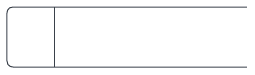
\includegraphics[width=0.2\textwidth]{Open_Rectangle.png}\\ Represents a data store.
\end{itemize}

\subsection{Level 0 DFD (Context Diagram) }
 
The Level 0 DFD provides a high-level overview of the system. It encapsulates the entire system as a single process and illustrates the interaction between the system and external entities. In the context of the chatbot application, the external entities could include the User and the Database (Postgres). The User interacts with the system (Chatbot Application) which in turn interacts with the Database.

\begin{figure}[h]
  \centering
  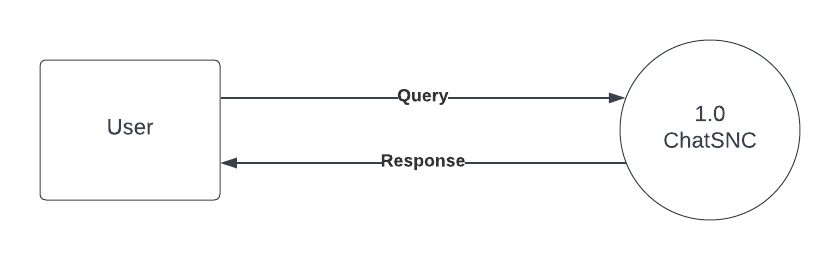
\includegraphics[width=.75\textwidth]{Level-0-DFD.png}
  \caption{Level 0 DFD}\label{fig:level-0-dfd}
\end{figure}

\subsection{Level 1 DFD}
The Level 1 DFD breaks down the main process of the Level 0 DFD into smaller sub-processes to provide a more detailed view of the system's operation. In the case of the chatbot application, the main process can be broken down into several sub-processes such as User Registration, User Login, Chat Generation, and Create/Update Chat History. Each of these sub-processes interacts with each other and with the Database to ensure the smooth operation of the chatbot application.

\begin{figure}[h]
  \centering
  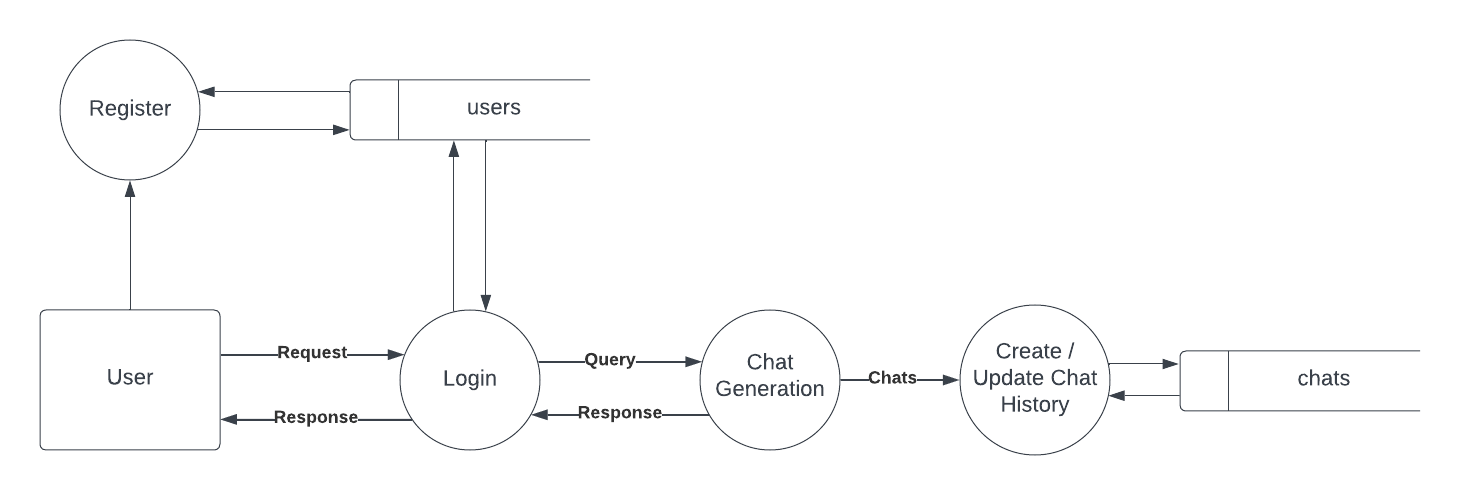
\includegraphics[width=\textwidth]{Level-1-DFD.png}
  \caption{Level 1 DFD}\label{fig:level-1-dfd}
\end{figure}

\section{Use Case Diagram}
The Use Case Diagram for the chatbot application provides a visual representation of the system's functionality from the user's perspective. It illustrates the different use cases or interactions that a user can have with the system. The Use Case Diagram typically consists of actors, use cases, and the relationships between them.

\begin{figure}[h!]
  \centering
  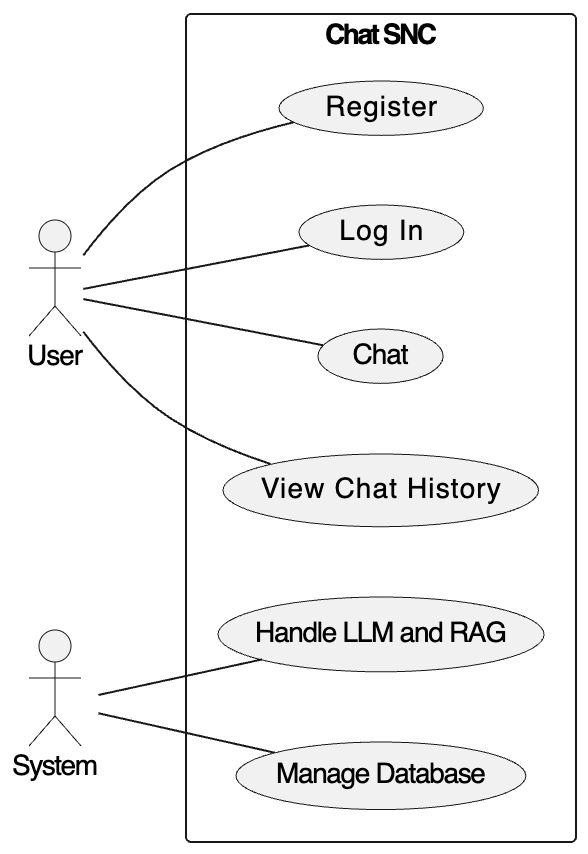
\includegraphics[width=.70\textwidth]{UseCase.png}
  \caption{Use Case Diagram}\label{fig:use-case-diagram}
\end{figure}

\subsection*{Actors}

\begin{itemize}
  \item \textbf{User}: The person interacting with the chatbot application.
  \item \textbf{Systen}: The chatbot application itself, which includes the backend (Python FastAPI), frontend (JavaScript Vue.js), and the database (Postgres).
\end{itemize}

\subsection*{Use Cases}

\begin{itemize}
  \item \textbf{User Registration}: This use case involves the user creating a new account in the system.
  \item \textbf{User Login}: This use case involves the user logging into the system using their credentials.
  \item \textbf{Chat Generation}: This use case involves the user interacting with the chatbot. 
  \item \textbf{View Chat History}: This use case involves the user viewing their past interactions with the chatbot.
  \item \textbf{Handle LLM and RAG}: This use case involves the system handling Language Model (LLM) and Retrieval Augmented Generation (RAG) to generate chat responses.
  \item \textbf{Manage Database}: This use case involves the system storing and retrieving user data and chat history from the Postgres database.
\end{itemize}

\section{Entity Relationship Diagram}

The Entity Relationship Diagram (ERD) for the application illustrates the relationship between two primary entities: \textit{users} and \textit{chats}, which are housed within a public schema.

\begin{figure}[h]
  \centering
  \includegraphics[width=\textwidth]{ERD.png}
  \caption{Entity Relationship Diagram}\label{fig:erd}
\end{figure}

\subsection*{Users Entity}

The \textit{users} entity contains the following attributes:

\begin{itemize}
  \item \textbf{id}: A unique identifier for each user.
  \item \textbf{email}: The email address of the user.
  \item \textbf{password}: The password of the user.
  \item \textbf{created\_at}: The timestamp of user creation.
\end{itemize}

\subsection*{Chats Entity}

The \textit{chats} entity contains the following attributes:

\begin{itemize}
  \item \textbf{id}: A unique identifier for each chat.
  \item \textbf{user\_id}: Acts as a foreign key, linking each chat to a specific user in the \textit{users} entity.
  \item \textbf{history}: Stores the chat history of the user.
  \item \textbf{created\_at}: The timestamp of chat creation.
\end{itemize}

\section{System Flowchart}

The system flowchart for the chatbot application outlines the user interaction process. Here's a description of the flowchart:

\begin{figure}[h!]
  \centering
  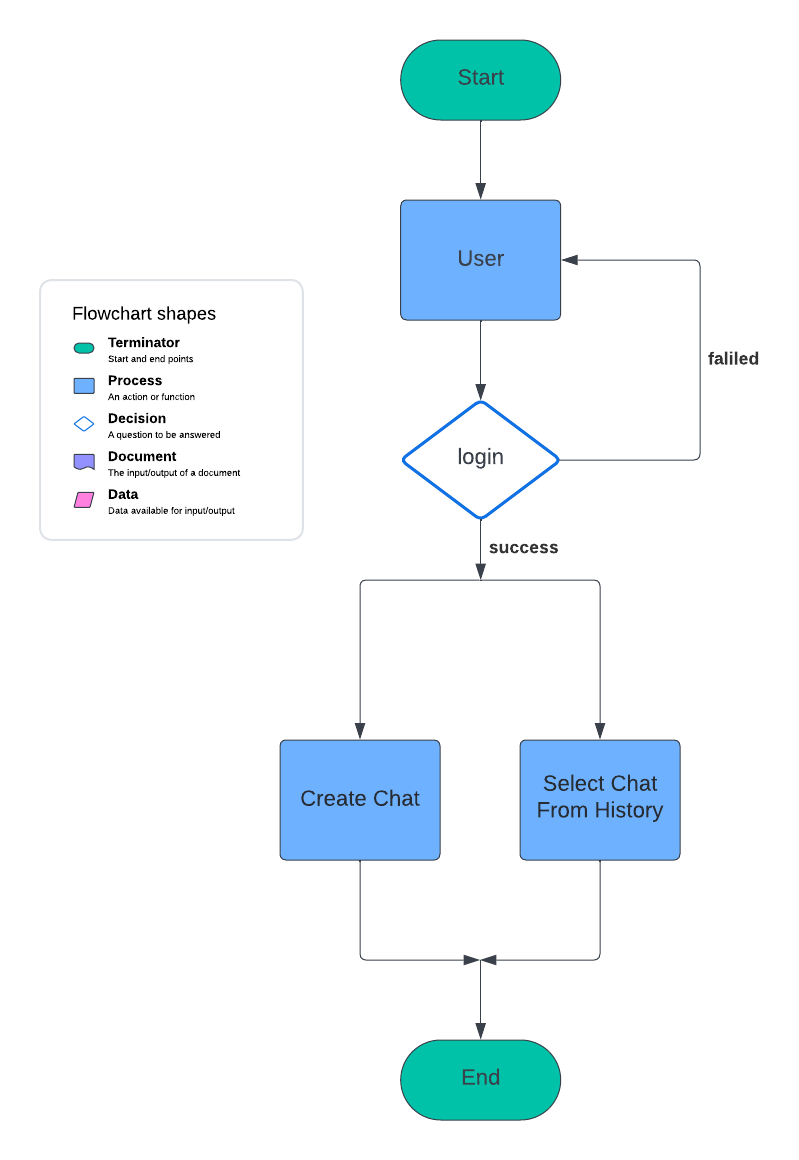
\includegraphics[width=.75\textwidth]{flowchart.png}
  \caption{System flowchart for user}\label{fig:flowchart}
\end{figure}

\begin{enumerate}
  \item \textbf{Start}: The process begins at the “Start” node.
  \item \textbf{User Interaction}: The user initiates interaction with the system.
  \item \textbf{Login}: The user attempts to log in. This is a decision-making point in the flow.
  \begin{itemize}
    \item If the login is successful, the process moves to the next step.
    \item If the login fails, the process loops back to the user for another login attempt.
  \end{itemize}
  \item \textbf{Post-Login Options}: After a successful login, the user has two options:
  \begin{itemize}
    \item Create a new chat.
    \item Select a chat from the chat history.
  \end{itemize}
  \item \textbf{End}: The flow ends after the user selects an option post-login..
\end{enumerate}
